\chapter{Literature Survey}
%
% Literature survey section provides an overview of prior research relevant to the current study.
% Paper 1: This entry details the key concepts of the paper on enhancing real-time object detection using the YOLO algorithm.
%
% Paper Title and Authors
{ \textbf{[2.1] \underline{{ENHANCING REAL-TIME OBJECT DETECTION WITH YOLO ALGOR-}} \\ \underline{ITHM}}}\newline
\newline
%
% Introduction to the paper: Brief overview of the purpose and importance of real-time object detection.
This paper titled \textbf{"Enhancing real-time object detection with YOLO algorithm"}, authored by \textbf{Gudala Lavanya and Sagar Dhanraj Pande}, focuses on the advancements in real-time object detection through the YOLO (You Only Look Once) algorithm. Real-time object detection plays a vital role in areas like video surveillance, autonomous vehicles, and robotics. Traditional detection methods often require multiple passes over images, which increases the processing time. The YOLO algorithm, treats object detection as a single-stage regression task, predicting bounding boxes and class probabilities in a single evaluation.\\\\
%
% Discussion on why YOLO is favored in the field, followed by the evolution of YOLO versions.
Due to its ability to detect objects in real-time with high accuracy, YOLO is highly regarded in the field of computer vision. The paper covers various versions of YOLO, highlighting their improvements in speed, accuracy, and handling of different object scales. YOLOv1 introduced a grid-based detection approach, while later versions incorporated anchor boxes, feature pyramids, and more sophisticated models like Darknet-53.\\\\
%
% Breakdown of the methodology used in YOLO for object detection.
\textbf{The methodology of YOLO involves:}
\begin{enumerate}
  % Step 1: Preprocessing the input image for uniformity.
  \item \textbf{Image Preprocessing:} The input image is resized to a uniform size.
  %
  % Step 2: Dividing the image into a grid for assigning detection responsibilities.
  \item \textbf{Grid Division:} The image is divided into a grid, with each cell responsible for predicting bounding boxes and class probabilities.
  %
  % Step 3: Bounding box prediction and class probability assignments.
  \item \textbf{Bounding Box Prediction:} The model predicts the center of each object within a grid cell and generates corresponding bounding boxes.
  %
  % Step 4: YOLO assigns class labels based on confidence scores for each detected object.
  \item \textbf{Class Label Assignment:} YOLO assigns class labels to detected objects based on confidence scores.
  \begin{itemize}
    % Explanation of confidence scores and their importance.
    \item \textbf{Confidence Score}: YOLO assigns a score to each bounding box, indicating the likelihood it contains an object.
    %
    % Details on class probability calculations for multiple classes.
    \item \textbf{Class Probabilities}: For each object, YOLO predicts probabilities for multiple classes (e.g., "car," "bus," "truck").
    %
    % Determining the final class label by choosing the highest probability.
    \item \textbf{Class Label Assignment}: The class with the highest probability is assigned to the object.
    \begin{itemize}
       % Example to clarify the class label assignment process.
       \item \textbf{Example}: If "car" = 0.8, "bus" = 0.6, and "truck" = 0.3, the object is labeled as "car."
    \end{itemize}
  \end{itemize}
  %
  % Step 5: Non-maximum suppression is used to refine detections by resolving overlapping bounding boxes.
  \item \textbf{Resolving Multiple Bounding Boxes:} Non-maximum suppression (NMS) is a fundamental technique YOLO employs to address this challenge.\\\\
  %
  % Explanation of steps in Non-Maximum Suppression (NMS) to avoid duplicate detections.
  \textbf{Steps in NMS:}
  \begin{enumerate}
    \item Select the box with the highest confidence score, denoted as $\hat{c}$.
    \item Compute the Intersection over Union (IoU) between this box and all other boxes of the same class.
    \item Remove boxes with an IoU greater than a set threshold (typically 0.5).
    \item Repeat the process with the next highest confidence box until all boxes are processed.
    \item The remaining boxes are the final detections.
  \end{enumerate}
\end{enumerate}
%
% Figure illustrating IoU (Intersection over Union) concept for bounding box refinement.
\begin{figure}[h!]
    \centering
    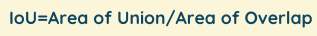
\includegraphics[width=0.5\textwidth]{images/IoU.png}
\end{figure}
%
% Figure illustrating the general steps involved in the YOLO algorithm.
\begin{figure}[h!]
    \centering
    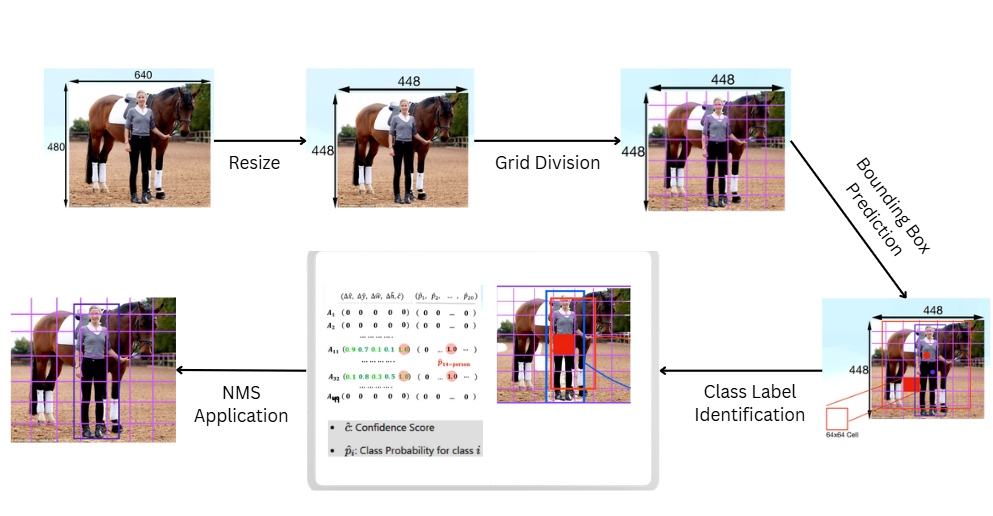
\includegraphics[width=1\textwidth]{images/Yolo Steps.png}
    \caption{Steps in YOLO}
\end{figure}
%
% Evaluation of YOLO model: performance assessment on standard datasets and its applicability to real-time scenarios.
The model was evaluated using standard datasets and achieved notable success due to its ability to process images in real-time, a key feature for applications that require immediate analysis of visual data.\\\\
%
% Conclusion emphasizing YOLO’s impact and continuous improvements over different versions.
The paper concludes by emphasizing YOLO's revolutionary impact on the field of real-time object detection. Its combination of speed and accuracy makes it a superior choice compared to traditional object detection methods. The continuous development across various versions (v1 to v8) has enhanced YOLO's ability to detect small objects, perform better on complex datasets, and improve overall detection efficiency.\\
%
% Figure showing the improvement and features added to each YOLO version over time.
\begin{figure}[h!]
    \centering
    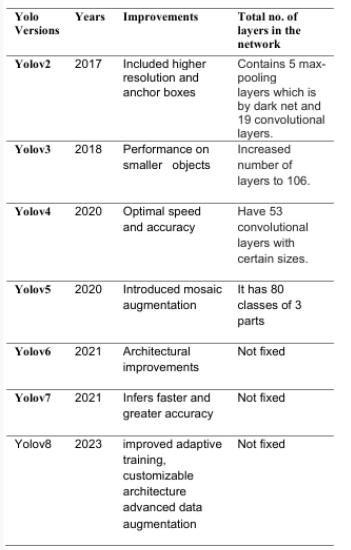
\includegraphics[width=0.8\textwidth]{images/YOLOv1 to YOLOv8.png}
    \caption{YOLO Versions Improvements Over Time}
\end{figure}\\\\
%
%
% Section for Paper 2 Title and Author Information
{ \textbf{[2.2] \underline{IMPROVED YOLOv8 MODEL FOR A COMPREHENSIVE APPROACH TO } \\ \underline{OBJECT DETECTION AND DISTANCE ESTIMATION} }
\\\\
%
% Title and Author Introduction
The paper titled \textbf{"Improved YOLOv8 Model for a Comprehensive Approach to Object Detection and Distance Estimation"}, authored by \textbf{Zu Jun Khow, Yi-Fei Tan, Hezerul Abdul Karim and Hairul Azhar Abdul Rashid}, proposes an enhanced object detection model called YOLOv8-CAW. This model builds on the YOLOv8 architecture and incorporates two key components: the Coordinate Attention (CA) module and the Wise-Intersection over Union (Wise-IoU) loss function, both of which work together to improve object detection accuracy and distance estimation.\\\\
%
% Research Objective
The primary aim of the research is to address limitations in current models, especially for small object detection and distance estimation within the field of computer vision. The methodology focuses on integrating the CA module, which enhances the model’s focus on crucial regions of the image without significantly increasing its size. This attention mechanism captures positional information in both horizontal and vertical directions, resulting in more precise object localization. Additionally, the Wise-IoU loss function further enhances the training process by dynamically adjusting loss coefficients for high and low-quality samples, leading to more accurate bounding box predictions.\\\\
%
% Figure: YOLOv8-CAW Model Architecture
\begin{figure}[h!]
    \centering
    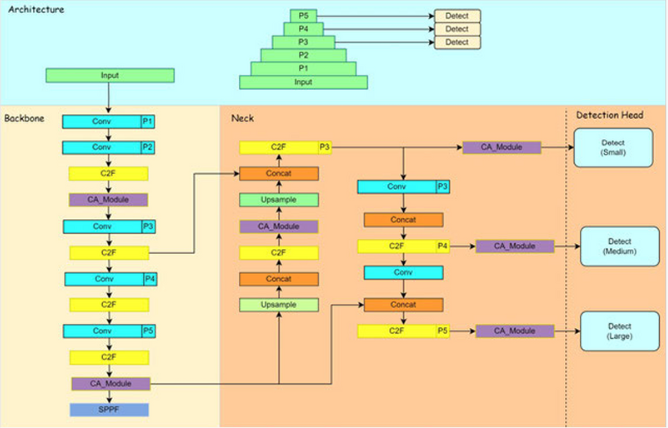
\includegraphics[width=0.7\textwidth]{images/YOLOv8 CAW Architecture.png}
    \caption{YOLOv8-CAW Model Architecture}
\end{figure}\\\\
%
% Distance Estimation Technique
Furthermore, the paper introduces a distance estimation technique, which calculates the distance between the camera and the detected object by comparing the real-world size of the object with its size in the captured image. This method achieves approximately 90\% accuracy based on experimental validation.\\\\
%
% Methodology Outline
\textbf{The methodology consists of three core steps:}
\begin{enumerate}
  % Step 1: Coordinate Attention Module
  \item \textbf{Coordinate Attention (CA) Module:} The CA module in YOLOv8-CAW enhances localization accuracy and detection performance by focusing on relevant regions of the feature map without significantly increasing model size. This advanced attention mechanism embeds positional information into channel attention, allowing the network to concentrate on critical areas efficiently.
\\\\
\textbf{Key Features:}
\begin{itemize}
    \item \textbf{Positional Information Embedding:} Helps the model identify important object locations in the image.
    \item \textbf{Efficient Computation:} Processes the image in horizontal and vertical directions to improve relationships between features and enhance accuracy.
    \item \textbf{Directional Attention Maps:} Generates separate maps for horizontal and vertical focus, refining the detection process further.\\
\end{itemize}
%  
% Figure: Coordinate Attention Equation
\begin{figure}[h!]
    \centering
    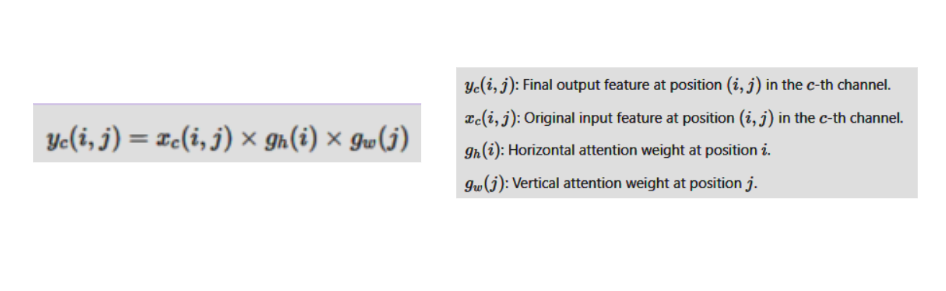
\includegraphics[width=1\textwidth]{images/CA Eqn.png}
\end{figure}
%
  % Step 2: Wise-IoU Loss Function
  \item \textbf{Wise-IoU Loss Function:} Enhances the accuracy of bounding box predictions by concentrating on the overlap between the predicted bounding boxes and the ground truth bounding boxes.\\\\
  %
  % Wise-IoU Loss Function Advantages
  \textbf{A. Advantages of Wise-IoU over IoU:}
\begin{itemize}
    \item \textbf{Emphasizes Overlap:} Prioritizes intersection areas for more accurate predictions.
    \item \textbf{Robust to Small Overlaps:} Handles small overlaps better, reducing penalties for minor discrepancies.
    \item \textbf{Focus on Localization:} Adjusts loss based on spatial distribution, improving bounding box predictions.\\
\end{itemize}
\textbf{B. How Wise-IoU Works:}
\begin{itemize}
    \item Calculates the intersection area between the predicted and ground truth boxes.
    \newpage
    \item Adjusts loss based on overlap degree, focusing on significant intersections.
    \item Encourages minimizing the distance between predicted and actual bounding boxes for better accuracy.
\end{itemize}
%  
% Figure: Wise-IoU Equation
\begin{figure}[h!]
    \centering
    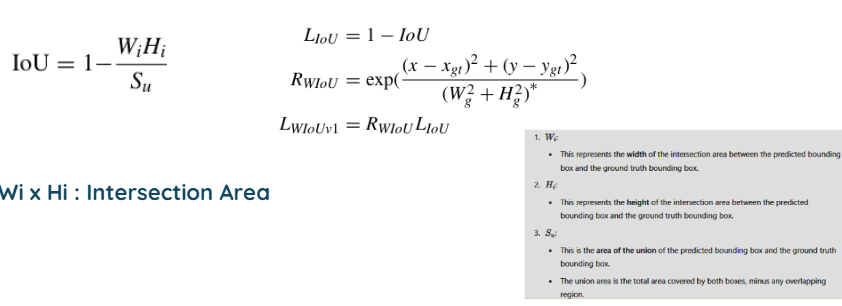
\includegraphics[width=1\textwidth]{images/WIoU Eqn.png}
\end{figure}
%
  % Step 3: Distance Estimation Algorithm
  \item \textbf{Distance Estimation Algorithm:} Uses the ratio calculation method to compare the average size of an object in the real world with its size in a captured image
\end{enumerate}
%  
% Figure: Distance Estimation Equation
\begin{figure}[h!]
    \centering
    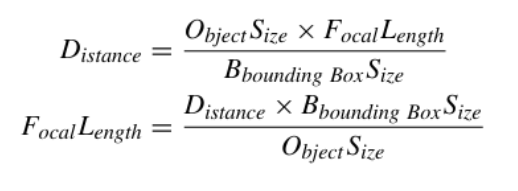
\includegraphics[width=0.5\textwidth]{images/Distance Estimation Eqn.png}
\end{figure}
%  
% 
\setlength{\fboxsep}{0pt} % Removes the padding around the image
\setlength{\fboxrule}{1pt} % Sets the thickness of the frame
%
% Figure: Distance Estimation Algorithm
\begin{figure}[h!]
    \centering
    \fbox{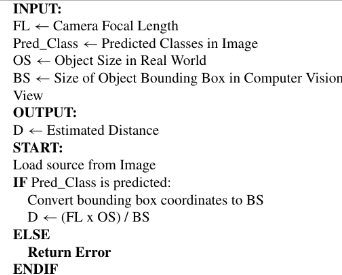
\includegraphics[width=0.5\textwidth]{images/Distance Estimation Algorithm.png}}
    \caption{Distance Estimation Algorithm}
\end{figure}
%
%
% Performance on Datasets
The model was tested on popular datasets like PASCAL VOC and MS-COCO, demonstrating improvements in recall, precision, and Mean Average Precision (mAP), with a particular focus on small object detection.\\\\
%
% Figure: YOLOv8-CAW Model vs Other Models
\begin{figure}[h!]
    \centering
    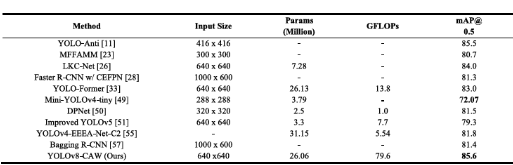
\includegraphics[width=1\textwidth]{images/YOLOv8-CAW vs Other Models.png}
    \caption{YOLOv8-CAW Model vs Other Model on Pascal VOC DataSet 2007}
\end{figure}
%
% Figure: Distance Estimation Result
\begin{figure}[h!]
    \centering
    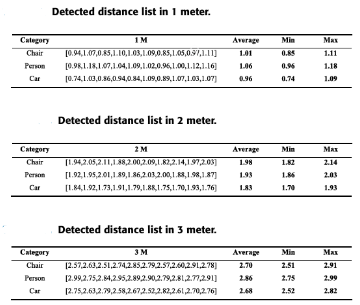
\includegraphics[width=0.8\textwidth]{images/Distance Estimation Result.png}
    \caption{Distance Estimation Result}
\end{figure}\\
%
%
% Section for Paper 3 Title and Author Information
\noindent
{\textbf{[2.3] \underline{AUTOMATED VEHICLE COUNTING FROM PRE-RECORDED VIDEO } \\ \underline{USING YOLO OBJECT DETECTION MODEL}}}\\\\
%
% Title and Author Introduction
The paper titled \textbf{"Automated vehicle counting from pre-recorded video using YOLO object detection model"}, authored by \textbf{Mishuk Majumder and Chester Wilmot}, introduces an automated method for vehicle counting using pre-recorded footage videos using the YOLOv3 (You Only Look Once) object detection model. Traffic monitoring is a critical component for urban planning, and traditional methods are often time-consuming and susceptible to errors. YOLOv3, with its capacity to identify objects in real-time, provides a more efficient solution to this problem.\\\\
%
% Research Objective and Dataset
The paper's primary objective is to develop algorithms for detecting, tracking, and counting vehicles in pre-recorded videos. The dataset used in this study consists of video recordings from ten strip mall business sites located in Baton Rouge, Louisiana, recorded over two consecutive days.\\\\
%
% Outline of Methodology Steps
\textbf{The methodology consists of the subsequent steps:}
\begin{enumerate}
  % Step 1: Data Collection and Pre-processing
  \item \textbf{Data Collection and Pre-processing:} Videos were collected and pre-processed, including frame extraction and resizing for uniformity.
  %
  % Step 2: YOLO Version Selection
  \item \textbf{YOLO Version Selection:} YOLOv3 was chosen due to its balance between speed and accuracy, making it ideal for real-time detection.
  %
  % Step 3: Conversion to TensorFlow API
  \item \textbf{Conversion to TensorFlow:} The YOLO weight file, originally in C/C++, was converted to the TensorFlow API to be used in Python. Python was preferred for its flexibility and ease of use in the project.
  %
  % Step 4: System Setup for YOLO and Video Files
  \item \textbf{Setup:} The necessary video files were prepared in .mp4 format and uploaded into the system. Relevant settings, including the YOLO model configuration, video file location, and system resources such as available GPUs, were specified. The system was then checked and prepared for vehicle detection.
  \begin{itemize}
    \item \textbf{YOLO Model Settings}: Specify the location of the YOLO weight file, configure model settings (e.g., detection thresholds), and check available GPUs for processing.
    \item \textbf{Video File Settings}: Configure the video file name and its location for vehicle detection. Ensure the video is in \texttt{.mp4} format.
    \item \textbf{Prepare Video}: Convert the video files to \texttt{.mp4} if necessary and merge multiple video files if needed, as the program processes only one file at a time.
    \item \textbf{Upload Video}: Drag and drop the \texttt{.mp4} video into the input section. Enter the video name (excluding the \texttt{.mp4} extension) into the program.
    \item \textbf{Check and Process}: Run the program to verify the input files and settings. Once verified, the vehicle detection process can begin.
  \end{itemize}
  %
  % Step 5: Reference Line Drawing and Vehicle Detection
  \item \textbf{Reference Line Drawing and Vehicle Detection:} Reference lines were manually drawn on video frames as allowed by the algorithm to mark areas for vehicle detection. YOLOv3 was then used to generate bounding boxes around the detected vehicles.
  %
  % Step 6: Vehicle Tracking using Kalman Box Tracker
  \item \textbf{Vehicle Tracking:} Vehicles were tracked across multiple frames using the Kalman Box Tracker, which compared pixel values between frames to keep track of the vehicles' locations. Each detected vehicle was assigned a unique ID for identification.
  \begin{itemize}
    \item \textbf{Tracking Objects}: To track vehicles across thousands of video frames, the program compares each frame with the previous one using pixel differences.
    \item \textbf{Kalman Box Tracker}: This algorithm tracks bounding boxes by checking for similarities in pixel values across frames, updating and memorizing the vehicle’s bounding boxes.
    \item \textbf{Identification and Display}: Each detected vehicle is assigned a unique numeric ID. Rectangles are drawn around tracked objects, and a dotted centerline is used to aid vehicle counting.
  \end{itemize}
  %
  % Step 7: Vehicle Counting with Direction Tracking
  \item \textbf{Vehicle Counting:} The direction of vehicle movement was determined based on whether it crossed the reference line from left to right (entry) or right to left (exit). Counters for both directions were maintained using custom algorithms.
  \begin{itemize}
    \item \textbf{Counting Directions}: The direction of vehicle movement is determined by whether the center point of the bounding box (BB) crosses the reference line:
    \begin{itemize}
        \item \textbf{Entry Count (L2R)}: Vehicles crossing from left to right (L2R) are counted as entering.
        \item \textbf{Exit Count (R2L)}: Vehicles crossing from right to left (R2L) are counted as exiting.
    \end{itemize}
    \item \textbf{Functions for Counting}:
    \begin{itemize}
        \item \texttt{leftToRight\_counter}: Tracks and counts vehicles entering from the left.
        \item \texttt{rightToLeft\_counter}: Tracks and counts vehicles exiting from the right.
    \end{itemize}
  \end{itemize}
  %
  % Step 8: Output Results and Display
  \item \textbf{Output:} The program outputs vehicle counts in both a spreadsheet and on-screen, with real-time adjustments for accurate tracking and customizable time intervals.
  \begin{itemize}
    \item \textbf{Output Format}: The program generates a spreadsheet displaying vehicle counts for each direction (entry or exit) over a flexible time interval.
    \item \textbf{Time Interval Adjustment}: YOLO calculates the number of frames and the processing time per frame to match real-time intervals. The YOLO time interval is adjusted accordingly for accurate counts.
    \item \textbf{Display}: Vehicle counts are displayed on the computer screen and in the spreadsheet, with detailed examples provided (e.g., entry and exit counts at locations such as strip malls).
  \end{itemize}
\end{enumerate}
%
% Figure: YOLO-Based Vehicle Detection and Center Line
\begin{figure}[h!]
    \centering
    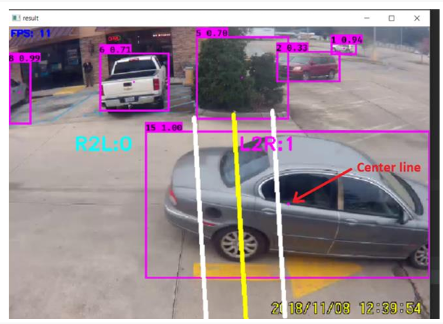
\includegraphics[width=0.4\textwidth]{images/Paper 3 Algorithm Implementation.png}
    \caption{YOLO-Based Vehicle Detection with Center Line and Direction Indicators}
\end{figure}
%
% Figure: Step-by-Step Process for Vehicle Detection
\begin{figure}[h!]
    \centering
    \fbox{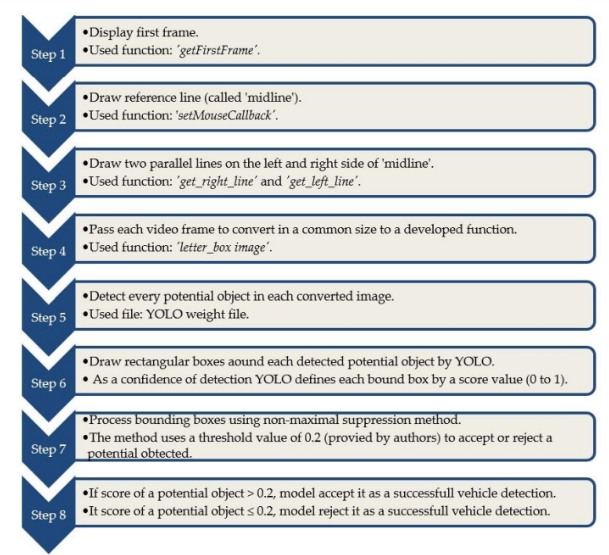
\includegraphics[width=0.8\textwidth]{images/Paper 3 Algorithm.png}}
    \caption{Step-by-Step Process for Vehicle Detection Using YOLO and Line Detection}
\end{figure}
%
% Output Results and Effectiveness
The results were outputted in a spreadsheet format that included vehicle counts over specified time intervals. The results were displayed in real-time on the screen as well as logged in the spreadsheet, with counts showing vehicles entering and exiting various locations such as strip malls. This study demonstrates the effectiveness of YOLOv3 for automating vehicle counting, providing a fast and reliable solution for traffic monitoring and urban planning purposes.\\\\
%
% Figure: Accuracy of Manual vs Automated Counts
\begin{figure}[h!]
    \centering
    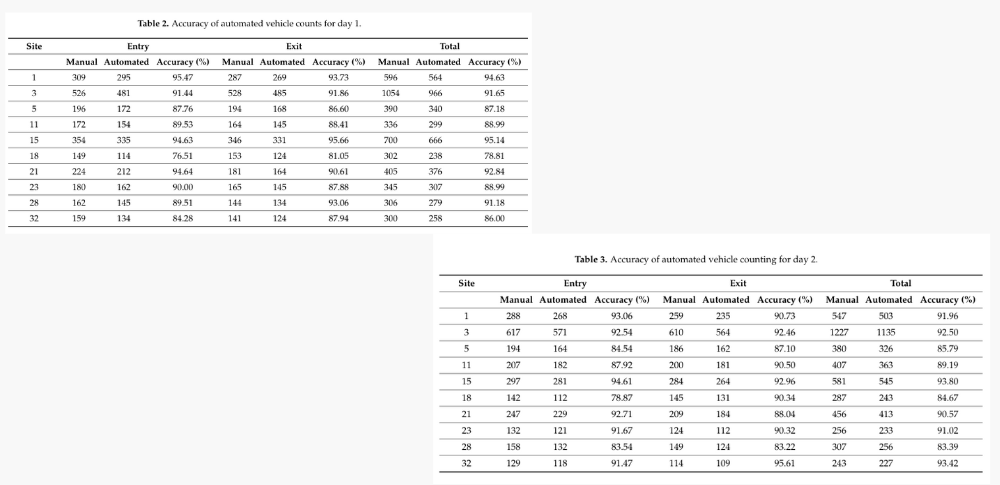
\includegraphics[width=0.8\textwidth]{images/Paper 3 Result.png}
    \caption{Accuracy of Manual vs Automated Vehicle Counts for Two Days}
\end{figure}
%
%
\newpage
\noindent
% Paper 4 - Modified YOLO for Object Tracking in Video
{\textbf{[2.4] \underline{MODIFIED YOLO MODULE FOR EFFICIENT OBJECT TRACKING IN} \\ \underline{A VIDEO}}}\\\\
%
% Summary of paper on Modified YOLO
The paper titled \textbf{"Modified YOLO Module for Efficient Object Tracking"}, authored by \textbf{Varsha Kshirsagar, Raghavendra Bhalerao, and Manish Chaturvedi}, proposes enhancements to the YOLO (You Only Look Once) algorithm to improve object tracking accuracy in video sequences. It addresses the challenges posed by fluctuations in confidence scores and misclassification of objects between consecutive frames, which often affect tracking and counting tasks, especially in complex environments like traffic monitoring.\\\\
%
% Original YOLO limitations
The original YOLO algorithm is widely recognized for its real-time object detection capabilities. However, it struggles with sudden drops in confidence scores across frames, leading to incorrect object classification and tracking inaccuracies. To overcome these limitations, the authors propose a modification that integrates RANSAC (Random Sample Consensus) algorithm and linear interpolation to smooth out confidence score fluctuations and improve overall tracking performance.
%
%
\begin{figure}[h!]
    \centering
    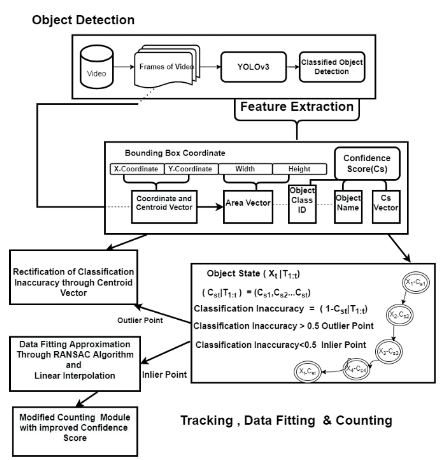
\includegraphics[width=0.8\textwidth]{images/Paper 4 Architecture.png}
    \caption{Enhanced Object Detection and Tracking Framework}
\end{figure}
%
%
\newpage
\noindent
% Key steps in methodology
\textbf{The methodology presented in the paper involves several key steps:}
\begin{enumerate}
  % Step 1: Object detection with YOLO
  \item \textbf{Object Detection Using YOLO:} The YOLO algorithm is employed for object detection across video frames. It uses bounding boxes, object class, and confidence scores to detect objects, particularly vehicles, in each frame.
  \begin{itemize}
    % YOLO's accuracy in single frames
    \item \textbf{YOLO's Strength in Single Frames:} YOLO's ability to perform well on single frames makes it particularly suitable for detecting objects accurately in each frame.
    % Use of YOLOv3 for vehicle detection
    \item \textbf{YOLOv3 for Vehicle Detection:} YOLOv3 is specifically used due to its effectiveness in detecting vehicles, making it ideal for tasks focused on identifying cars, buses, and other vehicles.
  \end{itemize}
  %
  % Step 2: Feature extraction
  \item \textbf{Feature Extraction:} Critical features such as object size, centroid coordinates, and confidence scores are extracted from the YOLO output. These features are essential for accurately tracking objects across frames.
  \begin{itemize}
      % Importance of YOLOv3 features
      \item \textbf{Key Features from YOLOv3:} YOLOv3 uses bounding box dimensions, centroid coordinates, object class, and confidence score for object detection and tracking.
      % Combining features for better accuracy
      \item \textbf{Importance of Multiple Features:} Combining features enhances tracking accuracy, especially when some features are unreliable in certain frames (e.g., due to occlusion).
      % Tracking parameters and their role
      \item \textbf{Tracking Parameters:} The extracted parameters, combined with the smooth centroid curve of the area, are used to track specific targets throughout the video.
  \end{itemize}
  %
  % Step 3: Outlier rejection and data fitting
  \item \textbf{Outlier Rejection and Data Fitting:} Outliers, or frames with drastic changes in confidence scores or misclassification, are identified and rejected using the \textbf{RANSAC} algorithm. To ensure a smoother confidence score trajectory across frames and maintain continuity in object tracking (Data Fitting), \textbf{Linear Interpolation} is applied to fill gaps caused by the rejected outliers.
  \begin{itemize}
      % Outlier detection process
      \item \textbf{Outlier:} Data points that significantly deviate from the norm; in this case, frames where the confidence score drops or object class changes unexpectedly.
      % Outlier detection based on confidence score
      \item \textbf{Identification:} Outliers are detected when confidence scores fall below a threshold or show abrupt variations.
      % Explanation of confidence score
      \item \textbf{Confidence Score (Cs):}
      \begin{itemize}
          % Definition and formula for confidence score
          \item \textbf{Definition:} Measures the certainty of object detection.
          \item \textbf{Formula:} 
          \[
          \text{Confidence Score} = Pr(\text{object}) \times IOU
          \]
          \item \textbf{Pr(object):} Probability of the object class \( 0 < Pr < 1 \)
          \item \textbf{IOU (Intersection over Union):} Overlap measure \( 0 < IOU < 1 \)
          \item \textbf{Max Value:} 1 (100\% confidence)
      \end{itemize}
      % Handling classification inaccuracies
      \item \textbf{Handling Classification Inaccuracy:}
      \begin{itemize}
          % Inaccuracy formula and threshold handling
          \item \textbf{Inaccuracy Formula:}
          \[
          1 = \text{ConfidenceScore} + \text{ClassificationInaccuracy}
          \]
          \item \textbf{Threshold Handling:} 
          \begin{itemize}
              \item If Inaccuracy \( > 0.5 \), retain previous class ID:
              \[
              \text{Class id}(n) = \text{Class id}(n-1)
              \]
              \item Replace outlier points with 0.
          \end{itemize}
      \end{itemize}
      % Tracking improvements
      \item \textbf{Tracking Improvements:}
      \begin{itemize}
          \item \textbf{RANSAC Algorithm:} Smooths tracking by identifying inliers and correcting outliers.
          \item \textbf{Linear Interpolation:} Fills gaps in confidence score data.
          \item \textbf{Area Consistency:} Object area should be 80-90\% of the previous frame’s area to maintain tracking.
      \end{itemize}
  \end{itemize}
  %
  % Step 4: Object tracking and counting
  \item \textbf{Object Tracking and Counting:} A and B represent the vehicle and marker line, with their index vectors denoted as ia and ib, respectively. 
%
%
\begin{figure}[h!]
    \centering
    \fbox{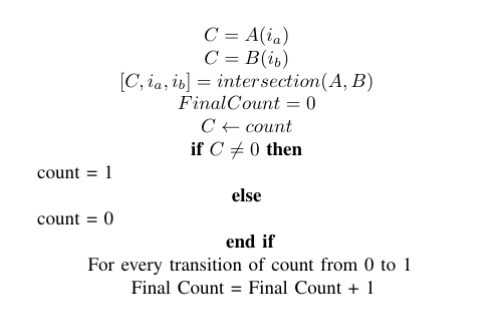
\includegraphics[width=0.8\textwidth]{images/Paper 4 Algorithm.png}}
    \caption{Object Counting Algorithm: Intersection-Based Counting Logic}
\end{figure}
%
%
\end{enumerate}
%
%
% Description of RANSAC algorithm
\textbf{RANSAC Algorithm}
\begin{itemize}
    \item The RANSAC algorithm minimizes the effect of outlier points and provides the best-fitted model with inlier points.
    \item The algorithm proposes a model from the extracted data, accounting for variations in confidence scores due to factors such as shadow and occlusion.
    \item RANSAC assists in finding a perfect curve from the extracted confidence score data obtained through YOLO.
\end{itemize}
%
%
\begin{figure}[h!]
    \centering
    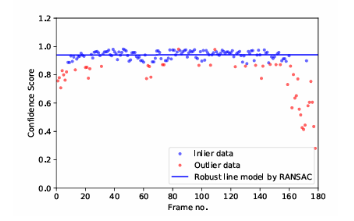
\includegraphics[width=0.8\textwidth]{images/RANSAC Outlier Rejection.png}
    \caption{Outlier Rejection by RANSAC algorithm}
\end{figure}
%
%
% Description of Linear Interpolation algorithm
\textbf{Linear Interpolation Algorithm}
\begin{itemize}
    \item Linear interpolation helps determine the closest point using the data from both outlier and inlier points obtained from the RANSAC approximation.
    \item At first, outlier points are substituted with zero.
    \item Then, linear interpolation is applied to replace these zeros with suitable values.
\end{itemize}
%
%
\begin{figure}[h!]
    \centering
    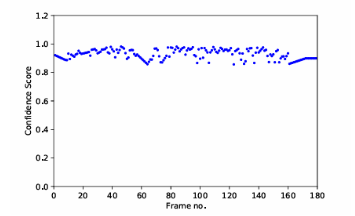
\includegraphics[width=0.8\textwidth]{images/Linear Interpolation.png}
    \caption{Track approximation by RANSAC and Linear Interpolation.}
\end{figure}
%
%
% Results of the modified YOLO module testing
The modified YOLO module was tested on custom traffic datasets and demonstrated significant improvements in object tracking and classification accuracy. Vehicle counting accuracy increased from 66\% to 87\%, and the overall classification accuracy ranged between 94\% and 96\%. This makes the proposed method highly effective for real-time applications, such as traffic monitoring and autonomous vehicle systems.\\\\
%
% Summary of YOLO framework enhancements
The integration of RANSAC and linear interpolation into the YOLO framework addresses key challenges in object tracking and classification, offering a robust solution for real-time applications. By maintaining consistent confidence scores and correcting misclassified frames, the modified YOLO module significantly improves both object tracking and counting accuracy. This enhancement makes it a valuable tool for video analysis tasks, especially in environments like traffic monitoring, where object tracking consistency is crucial.\\\\
%
%
%
%
\begin{figure}[h!]
    \centering
    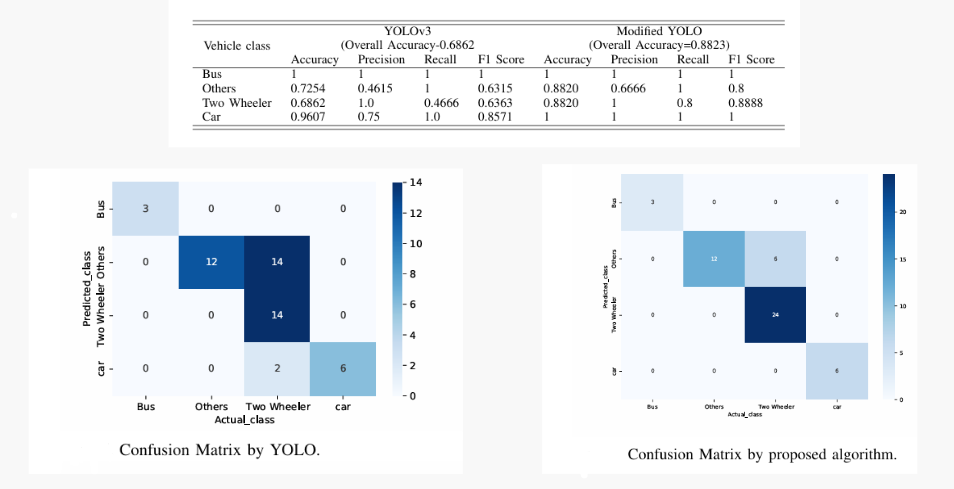
\includegraphics[width=1\textwidth]{images/Comparison of YOLOv3 and Modified YOLO Performance.png}
    \caption{Comparison of YOLOv3 \& Modified YOLO with RANSAC and Linear Interpolation}
\end{figure}
%
% End of the chapter
%
%